\section{Markov goes to Las Vegas}

Remember from last lecture that we saw two types of randomised algorithms: {Las Vegas} and {Monte Carlo}.\marginnote{There are more, of course: \eg Bellagio algorithms. And others! Mathematicians and computer scientists clearly love gambling~--~look up Jacob Bernoulli when you have a chance.}

\begin{quote}
\begin{description}
    \item[Las Vegas algorithms:] the algorithm is \emph{always correct}, but the running time is only bounded \emph{in expectation}. 
    \item[Monte-Carlo algorithms:] the algorithm is only \emph{correct with high probability}, but the running time is bounded \emph{with probability one}. 
\end{description}
\end{quote}
Wouldn't it be nice if there was a way to go from one to the other? Well, as it turns out, there is:
\begin{lemma}
    \label{lemma:lvtomc}
    Suppose there exists a Las Vegas algorithm $\Algo$ for some task, with expected running time $\blue{T}$. Then there exists a Monte Carlo algorithm $\Algo'$ for the same task with \emph{worst-case} running time $O(\blue{T})$ and probability of failure $1/100$.
\end{lemma}
\begin{proof}
The proof is quite simple, and relies on analyzing the following:
\begin{algorithm}[H]
\begin{algorithmic}[1]
    \Require input $x$
    \State Run $\Algo$ on $x$ for at most $100\blue{T}$ steps
    \If{$\Algo$ terminated within $100\blue{T}$ steps}
        \State\label{markov:line:goodoutput}\Return $\Algo$'s output \Comment{Always correct}
    \Else 
        \State\label{markov:line:mehoutput}\Return an arbitrary output \Comment{Very likely wrong}
    \EndIf
\end{algorithmic}
    \caption{Algorithm $\Algo'$.}
\end{algorithm}
It should be quite clear that the above algorithm always runs in time at most $100\blue{T} + O(1) = O(\blue{T})$; and also that whenever we reach~\cref{markov:line:goodoutput}, the output of $\Algo'$ must be correct (because $\Algo$, once it terminates, is always correct). 

When we reach~\cref{markov:line:mehoutput} because $\Algo$ ``timed out,'' however, we cannot really say anything: maybe what we output is correct, but it's most likely wrong. So we'll just assume it's an incorrect output, and all we need to do to prove the lemma is to prove that $\Algo$ ``times out'' with probability at most $1/100$.

Importantly, all we can use to do so is what we know about $\Algo$, which is very little: we only know its expected running time is at most $\blue{T}$, and that running times are non-negative. That's not a lot to build on, but that's just enough for \emph{Markov's inequality}:

\begin{theorem}[Markov's inequality]
Let $X$ be a non-negative\marginnote{The ``non-negative'' assumption is crucial. It is definitely not true without!} random variable with $\bEE{X} < \infty$. For any $t > 0$, we have
\[  
  \bPr{ X \geq t } \leq \frac{\bEE{X}}{t}
\]
\end{theorem}
\noindent Applying this with $X$ being the running time of $\Algo$ and $t=100$ proves the lemma.
\end{proof}
\marginnote{Lecture cue: prove Markov's.}
%%%
% Should I mention the algorithmic Jensen paper?
%%%
\section{Markov and beyond: Randomised Median}
% Useful/good: https://www.cs.dartmouth.edu/~deepc/LecNotes/Rand/lec6.pdf
As mentioned in the previous lecture, there exists a very neat, highly non-trivial (deterministic) divide-and-conquer algorithm to find the median of (an array of) $\ns$ numbers in linear time. You have seen it in previous  So we will not analyze it again: instead, we will give a simple (Monte Carlo) randomized algorithm, also linear-time. 

The idea of the algorithm is relatively simple, yet surprisingly powerful: given as input an array $\red{A}$ of $\ns$ integers\marginnote{For simplicity, we will throughout assume $\ns$ is odd, and that all numbers are distinct. Neither of these assumptions is necessary.}, subsample at random a \emph{smaller} array $\orange{B}$ of $\orange{m} \ll \ns$ integers from $\red{A}$, and use $\orange{B}$ as some sort of ``guide'' for what is in $\red{A}$. In particular, we expect, if we are not too unlucky, that finding ``approximate medians'' of $\orange{B}$ will give us an approximate idea of what the median of $\red{A}$ is, and we can then filter out a lot of the elements of $\red{A}$ to end up with a much more manageable task. And we can easily find that in $\orange{B}$, since it will have much smaller size!

Here is the actual algorithm, only missing the value of $\orange{m}$ (to be determined shortly):
\begin{algorithm}[H]
\begin{algorithmic}[1]
    \Require array $\red{A}$ of $\ns$ distinct integers
    \State Set $\Delta = 4\sqrt{\orange{m}}$ \Comment{Why? We'll see later. ``Chebyshev.''}
    \State Create an array $\orange{B}$ containing $\orange{m}$ elements of $\red{A}$ chosen independently and uniformly at random (with replacement)
    \State Sort $\orange{B}$ \Comment{Time $O(\orange{m}\log \orange{m})$}
    \State Let $\underline{b}$ and $\overline{b}$ be the $(\orange{m}/2-\Delta)$-th and $(\orange{m}/2+\Delta)$-th elements of $\orange{B}$ \Comment{``Approximate medians'' of $\orange{B}$}
    \State \Comment{Now we use $\underline{b}$ and $\overline{b}$ as ``guides'' for the contents of $\red{A}$. All 3 steps below take time $O(\ns)$.}
    \State\label{step:lintime:1} Copy every $x$ of $\red{A}$ with $\underline{b}\leq x\leq \overline{b}$ in a new array $\blue{C}$
    \State\label{step:lintime:2} Compute the number $k$ of elements of $\red{A}$ smaller than $\underline{b}$ 
    \State\label{step:lintime:3} Compute the number $\ell$ of elements of $\red{A}$ larger than $\overline{b}$ 
    \If{$k > \frac{\ns}{2}$ or $\ell > \frac{\ns}{2}$}
        \State\Return \textsf{fail} \Comment{The median of $\red{A}$ cannot be in $\blue{C}$}
    \ElsIf{$|\blue{C}| > \frac{4\ns\Delta}{\orange{m}}+2$}
        \State\Return \textsf{fail} \Comment{We cannot process $\blue{C}$ fast enough!}
    \Else
        \State Sort $\blue{C}$  \Comment{Time $O\big(\frac{\ns}{\sqrt{\orange{m}}}\log \frac{\ns}{\sqrt{\orange{m}}}\big)$}
        \State\label{step:return:median}\Return the $(\frac{\ns+1}{2}-k)$-th element of $\blue{C}$.
    \EndIf
\end{algorithmic}
    \caption{Randomised Median in Worst-Case Linear Time.}
    \label{algo:randomized:median}
\end{algorithm}

First, let's look at the time complexity. Assuming for now that $\orange{m} = \bigO{\ns/\log\ns}$ and $\frac{4\ns\Delta}{\orange{m}} = \bigO{\ns/\log\ns}$ (they will be!), the total time is dominated by~\cref{step:lintime:1,step:lintime:2,step:lintime:3}, and so the algorithm runs in (worst-case) time $O(\ns)$. Good.

Second, let's look at the correctness. Suppose the algorithm reaches~\cref{step:return:median}: then it not hard to see that the element returned is at position $k+\frac{\ns+1}{2}-k = \frac{\ns+1}{2}$ in $\red{A}$: that is, it indeed returns the median. 

So the algorithm always runs in time $O(\ns)$, and when it does not output \textsf{fail} it correctly outputs the median of $\red{A}$. This only leaves us with the third point: \emph{what is the probability the algorithm returns \textsf{fail}?}

This can only happen because of three things (``bad events''):
\begin{description}
    \item[Event ${E}_1$:] Too many elements are smaller than $\underline{b}$: $k > \frac{\ns}{2}$
    \item[Event ${E}_2$:]  Too many elements are larger than $\overline{b}$: $\ell > \frac{\ns}{2}$
    \item[Event ${E}_3$:]  $\blue{C}$ is too large: $|\blue{C}| > \frac{4\ns\Delta}{\orange{m}}+2$\marginnote{Why is that an issue, again?}
\end{description}
We want to get an upper bound on the probability \emph{at least one} of these three events occurs. We could try to argue these events are independent (maybe?) and try to bound $\probaOf{E_1\cup E_2\cup E_3} = 1-\probaOf{\overline{E_1}\cap\overline{E_2}\cap\overline{E_3}}$, and maybe (?) get some reasonable bound as a result. But independence is tricky to reason about, and nobody wants to do that if they do not have to. So instead, we will use the \emph{union bound}:\marginnote{The union bound sounds basic, but it is truly a fundamental, powerful tool.}
\begin{lemma}[Union Bound]
Let $E_1,\dots,E_k,\dots$ be a (possibly countably infinite) family of (possibly dependent) events. Then
\[
    \probaOf{ \bigcup_{k=1}^\infty E_k } \leq \sum_{k=1}^\infty \probaOf{E_k}\,. 
\]
\end{lemma}
This is great! No need to worry about independence: now we immediately have by the union bound that
\begin{equation}
    \label{eq:first:union:bound}
    \probaOf{E_1\cup E_2\cup E_3} \leq \probaOf{E_1}+\probaOf{E_2}+\probaOf{E_3}\,.
\end{equation}
By symmetry, one can also convince themselves that $\probaOf{E_1}=\probaOf{E_2}$, so we only have two things to analyze.

\paragraph{Bounding $\probaOf{E_1}$.} What is the probability that $k$, the number of elements of $\red{A}$ smaller than $\underline{b}$, exceeds $\frac{\ns}{2}$? By definition, if it exceeds $\frac{\ns}{2}$, then $\underline{b}$ is larger than (or equal to) the median of $\red{A}$. But $\underline{b}$ is the $(\frac{\orange{m}}{2} - \Delta)$-th element of $\orange{B}$, which means that among the $\orange{m}$ elements we picked uniformly at random (with replacement) to create $\orange{B}$, at most $\frac{\orange{m}}{2} - \Delta$ were smaller than the median.

Which should be unlikely: when we pick \emph{one} element uniformly at random from $\red{A}$, the probability to get an element smaller than the median is exactly $\frac{\ns-1}{2}\cdot \frac{1}{\ns} = \frac{1}{2} - \frac{1}{2\ns}$. So ``by linearity of expectation'' the expected number of elements smaller than the median is $\frac{\orange{m}}{2} - \frac{\orange{m}}{2\ns}$. But $\frac{\orange{m}}{2} - \Delta$, that's \emph{much} smaller than that! Can we quantify this?

Thankfully yes. Let's call ``the expected number of elements smaller than the median'' $X$. Then we can write $X = \sum_{i=1}^{\orange{m}} X_i$, where $X_i\in\{0,1\}$ is the indicator random variable for ``the $i$-th element sampled to go into $\orange{B}$ was smaller than the median of $\red{A}$.'' That is, all $X_i$s are \iid, and Bernoulli random variables with parameter $p \eqdef \frac{1}{2} - \frac{1}{2\ns}$,\marginnote{This means $X$ is a {Binomial} random variables with parameters $\orange{m}$ and $p$: $X\sim \binomial{\orange{m}}{p}$.} and so from what we saw about Binomials last week we get that $\var[X] = \orange{m}p(1-p) = \frac{\orange{m}}{4}\left(1-\frac{1}{\ns^2}\right) < \frac{\orange{m}}{4}$.

Why are we interested in the variance? Good question! We want to argue that most of the time $X$ is ``not too far from its expectation'' $\frac{\orange{m}}{2}\left(1-\frac{1}{\ns}\right)$, and in particular that getting as low as $\frac{\orange{m}}{2} - \Delta = \frac{\orange{m}}{2}\big(1 - \frac{2}{\sqrt{\orange{m}}}\big)$ is truly a freak event.\marginnote{Do it: try and apply Markov's inequality to $X$. Why doesn't it work? Then try to apply it to $\orange{m}-X$: why is the result too weak?} Unfortunately, using Markov's inequality here will not be enough\dots{} we need something stronger. 

And that's where \emph{Chebyshev's inequality} comes into play: instead of just using the expectation, Chebyshev allows you to leverage additional information you may have about the random variable, specifically its variance, to (usually) get stronger bounds:
\begin{theorem}[Chebyshev's inequality]
Let $X$ be a random variable with $\bEE{X^2} < \infty$. For any $t > 0$, we have
\[  
  \bPr{ \abs{X-\bEE{X}} \geq t } \leq \frac{\var[X]}{t^2}
\]
\end{theorem}
Another way to look at it: this is saying that a random variable usually may fluctuate around its expectation by give or take a few standard deviations (\ie a few $\sqrt{\var}$)\dots{} but \emph{more}? That's unlikely. \marginnote{By the way, this is why we set $\Delta = 4\sqrt{\orange{m}}$: the standard deviation of $X$ we computed about is $\approx \sqrt{\orange{m}}/2$, so that's the right order of magnitude.}


\begin{framed}
\noindent Compared to Markov's inequality, Chebyshev's:
\begin{itemize}
    \item Provides \emph{two-sided} bounds (bounds the probability to deviate too far below \emph{and} too far above the expectation) \hfill $\checkmark$
    \item Gives a bound that decays quadratically ($\propto 1/t^2$) instead of linearly ($\propto 1/t$), so is better for $t\geq 1$ (\cref{fig:markov:chebyshev}) \hfill $\checkmark$
    \item Does not require the random variable to be non-negative \hfill $\checkmark$
    \item Requires knowing a bound on the variance (if it exists) \hfill$\times$
\end{itemize}
\end{framed}
\begin{figure}[h]
    \centering
    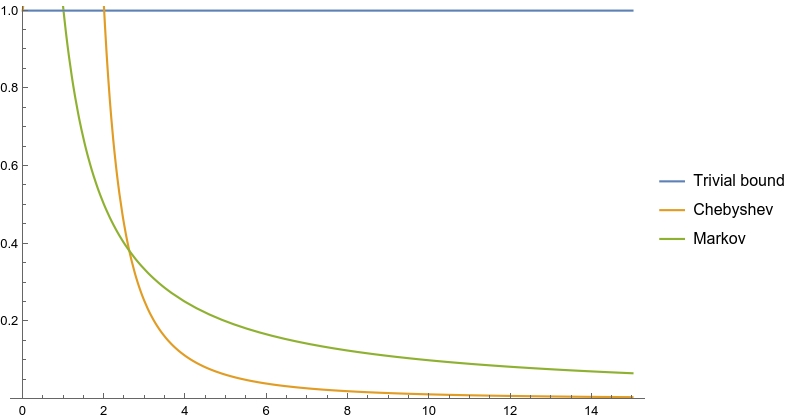
\includegraphics[width=0.9\textwidth]{figures/fig-markov-v-chebyshev.png}
    \caption{An illustration of the tail bounds $\probaOf{X\geq t}$ (as a function of $t\geq 0$) given by Markov and Chebyshev's inequalities, for the specific case of a non-negative random variable $X\geq 0$ with both expectation and variance equal to $1$: $\expect{X}=\var[X]=1$. Note that Chebyshev does not require that $X\geq 0$, this is simply here for the sake of comparison with Markov's inequality, which does.}
    \label{fig:markov:chebyshev}
\end{figure}
So we want to use Chebyshev's inequality to argue $\probaOf{X \leq \frac{\orange{m}}{2} - \Delta}$ is small. Here we go: rewriting $\frac{\orange{m}}{2} - \Delta = \expect{X} - \left(\Delta - \frac{\orange{m}}{2\ns}\right)$ and using $\orange{m}\leq \ns$ (so $\Delta - \frac{\orange{m}}{2\ns} \geq \Delta - \frac{1}{2} \geq \frac{\Delta}{2} = 2\sqrt{\orange{m}}$), we have
\begin{align*}
    \probaOf{X \leq \frac{\orange{m}}{2} - \Delta}
    &= \probaOf{X \leq \expect{X} - \left(\Delta - \frac{\orange{m}}{2\ns}\right)}\\
    &\leq \probaOf{\abs{X-\expect{X}} \geq \left(\Delta - \frac{\orange{m}}{2\ns}\right)}\\
    &\leq \frac{\var[X]}{\big(\Delta - \frac{\orange{m}}{2\ns}\big)^2} \tag{by Chebyshev}\\
    &\leq \frac{\orange{m}}{4(\Delta/2)^2} \tag{Bound on variance}\\
    &= \frac{1}{16} \tag{Setting of $\Delta$} 
\end{align*}
This gives us
\begin{equation}
    \label{eq:bounding:approxmedians:1}
    \probaOf{E_1},\probaOf{E_2} \leq \frac{1}{16}\,,
\end{equation}
using Chebyshev's inequality. We only have to bound $\probaOf{E_3}$ to conclude.

\paragraph{Bounding $\probaOf{E_3}$.} This is the last piece:\footnote{For now at last: there will be more down the line.} we want to bound the probability that $\blue{C}$ is ``too large,'' that is the probability $|\blue{C}|$ exceeds $4\orange{m}$. Since all we have seen so far relies either on computing the expectation of the quantity of interest, its variance, or both, it would seem reasonable to start with computing $\expect{|\blue{C}|}$ and maybe use Markov's inequality: unfortunately,
the quantity $\expect{|\blue{C}|}$ is quite tricky to compute. 

Instead, we will take an alternative path: let $R_{\underline{b}}$ denote the rank of $\underline{b}$ in $\red{A}$ (and similarly $R_{\overline{b}}$ for $\overline{b}$). We have already proven that 
\[
\probaOf{ R_{\underline{b}} > \frac{\ns}{2}} , \probaOf{ R_{\overline{b}} < \frac{\ns}{2}} \leq \frac{1}{16}
\]
(this is~\cref{eq:bounding:approxmedians:1}). Now, we want to prove that $|\blue{C}| = R_{\overline{b}}-R_{\underline{b}} +2 \leq \frac{4\ns\Delta}{\orange{m}}+2$ with high probability: so it'd \emph{suffice} to show that 
\[
\probaOf{ R_{\underline{b}} < \frac{\ns}{2} - 2\frac{\ns\Delta}{\orange{m}}} , \probaOf{ R_{\overline{b}} > \frac{\ns}{2} + 2\frac{\ns\Delta}{\orange{m}}} \leq \frac{1}{32}
\]
as this would imply the result. One may ask: \emph{why these particular values?} The reason is that since $\underline{b}$ is defined as the ($\frac{\orange{m}}{2} - \Delta$)-th element in $\orange{B}$, if the uniform random sampling was ``representative'' enough we expect to have an $\frac{1}{2} - \frac{\Delta}{\orange{m}}$ fraction of the original array $\red{A}$ on its left: so having much less than that, say a fraction $\frac{1}{2} - 2\frac{\Delta}{\orange{m}}$, ``should'' be unlikely.

As before, we will only focus on bounding $\probaOf{ R_{\underline{b}} < \frac{\ns}{2} - 2\frac{\ns\Delta}{\orange{m}}}$, as the case of $R_{\overline{b}}$ is similar (by symmetry). 

To proceed, let's consider the set $S$ of the $s\eqdef \frac{\ns}{2} - 2\frac{\ns\Delta}{\orange{m}}$ smallest elements of $\red{A}$~--~let's call them ``tail elements''. The key observation is that if \emph{fewer} than $\frac{\orange{m}}{2}-\Delta$ elements of $S$ end up in $\orange{B}$, then $\underline{b}$, being the ($\frac{\orange{m}}{2}-\Delta$)-th element of $\orange{B}$, is not a tail element: and so must have $R_{\underline{b}} \geq s$. Based on that, we want to show that the probability to have \emph{at least} $\frac{\orange{m}}{2}-\Delta$ of $S$ in $\orange{B}$ is small.

Now this looks familiar: the probability to pick an element of $S$ when choosing one from $\red{A}$ uniform at random is $\frac{s}{\ns} = \frac{1}{2} - \frac{2\Delta}{\orange{m}}$. The number of elements from $S$ in $\orange{B}$ (call it $Y$) is then a Binomial random variable with parameters $\orange{m}$ and $\frac{s}{\ns}$. We have $\expect{Y} = \frac{\orange{m}s}{\ns} = \frac{\orange{m}}{2}-2\Delta$, $\var[Y] = \frac{\orange{m}s}{\ns}\Paren{1-\frac{s}{\ns}} \leq \frac{\orange{m}s}{\ns} \leq \frac{\orange{m}}{2}$; and we want to bound
\begin{align*}
    \probaOf{Y \geq \frac{\orange{m}}{2}-\Delta}
    &= \probaOf{Y \geq \expect{Y}+\Delta} \\
    &\leq  \probaOf{|Y - \expect{Y}| \geq \Delta} \\
    &\leq \frac{\var[Y]}{\Delta^2} \tag{Chebyshev}\\
    &= \frac{\orange{m}}{2\cdot 16\orange{m}} \tag{as $\Delta= 4\sqrt{\orange{m}}$}\\
    &= \frac{1}{32}
\end{align*}
To summarize, we've just shown that
\[
    \probaOf{ R_{\underline{b}} < \frac{\ns}{2} - 2\frac{\ns\Delta}{\orange{m}}} \leq \probaOf{Y \geq \frac{\orange{m}}{2}-\Delta} \leq \frac{1}{32}
\]
We can similarly get $\probaOf{ R_{\overline{b}} > \frac{\ns}{2} + 2\frac{\ns\Delta}{\orange{m}}} \leq \frac{1}{32}$\marginnote{Do it! That's good practice.}, and so, ``by a union bound,''
\begin{align}
    \probaOf{E_3} &= \probaOf{|\blue{C}| > \frac{4\ns\Delta}{\orange{m}} + 2} \notag\\
    &\leq \probaOf{ R_{\underline{b}} < \frac{\ns}{2} - 2\frac{\ns\Delta}{\orange{m}}} + \probaOf{ R_{\overline{b}} > \frac{\ns}{2} + 2\frac{\ns\Delta}{\orange{m}}} \notag\\
    &\leq \frac{1}{16}\,.
\end{align}

\paragraph{Putting it together.}
The probability that the algorithm fails is bounded, from~\cref{eq:first:union:bound}, by
\[
\probaOf{E_1\cup E_2\cup E_3} \leq \probaOf{E_1}+\probaOf{E_2}+\probaOf{E_3} \leq \frac{1}{16} + \frac{1}{16} + \frac{1}{16} = \frac{3}{16}\,.
\]
When it doesn't fail, we have seen that it is correct; and it \emph{always} runs in time at most $O(\ns)$. So\dots{} we're done! \emph{Almost.} We haven't chosen the value of $\orange{m}$ yet!

So what do we need? For our running time, we need both $O(\orange{m}\log\orange{m})$ and $O(\frac{\ns\Delta}{\orange{m}}\log\frac{\ns\Delta}{\orange{m}}) =O(\frac{\ns}{\sqrt{\orange{m}}}\log \frac{\ns}{\sqrt{\orange{m}}})$ to be $O(\ns)$. There are many ways to do so, but one aesthetically pleasing choice is to make both equal:
\[
    \orange{m} = \frac{\ns}{\sqrt{\orange{m}}}
\]
which leads to setting $\boxed{\orange{m} = \ns^{2/3}}$. To conclude:
\begin{theorem}
    \label{theo:randomized:median}
    Randomised Median (\cref{algo:randomized:median}) is a linear-time Monte Carlo algorithm with failure probability at most $3/16$.
\end{theorem}

\section{But can we bring down this failure probability?}
This is all very good, but, when you think about it, a failure probability of $3/16\approx 19\%$ might be too much for many applications. Can we somehow bring this down to $1\%$? $0.01\%$? $\errprob$, for any $\errprob\in(0,1]$ of our choosing?

The obvious natural approach would be to go back to our analysis, see what the bottlenecks were, and modify the parameters to achieve smaller error probability. This would work \emph{here}\marginnote{\advancedstuff{} Go through the argument and see what happens to the probability of failure when you choose a larger $\Delta$, for instance $\orange{m}^{3/4}$ or $\sqrt{\ns}$.}, but it may not \emph{always} work, and honestly it is also very inconvenient. We went through a lot of trouble to establish~\cref{theo:randomized:median}, it would be nice not to have to start all over again!

Fortunately, it \emph{is} possible: there is a way to take our algorithm (and the guarantees we proved for it), and amplify its success probability \emph{in a blackbox way}. Of course, there is a cost: we will need to run the algorithm several times~--~the price is more computation time, and more random bits.\marginnote{Random bits are not always cheap: they are a resource, like time, and memory.}

Here is the idea: given the input array $\red{A}$ run the algorithm (\cref{algo:randomized:median}) $T$ times on $\red{A}$, using fresh (independent) random bits each time. If at any point the algorithm does not return $\textsf{fail}$, then return the median it outputs. If this never happens, return $\textsf{fail}$.

Since we have a Monte Carlo algorithm, whenever we return something else than $\textsf{fail}$ this is guaranteed to be correct, and we have the median. So what is the probability to output $\textsf{fail}$ now? Well, we need \emph{all} $T$ independent runs to fail. And they are all independent, so the probability that they all fail is at most
\[
    \Paren{\frac{3}{16}}^T
\]
Solving for this to be less than $\errprob$, we get that  taking
\[
    T = \clg{\frac{\log(1/\errprob)}{\log\frac{16}{3}}} = O(\log(1/\errprob))
\]
suffices. This gives the following:
\begin{corollary}
    \label{coro:randomized:median}
    For any $\errprob \in(0,1]$, the Repeated Randomised Median described above is a Monte Carlo algorithm with failure probability at most $\errprob$ and worst-case time complexity $O(\ns\log(1/\errprob))$.
\end{corollary}
\noindent This simple ``trick'' is your first example of \emph{probability amplification.}

\section{Viva Las Vegas!}
In light of~\cref{coro:randomized:median}, it is natural to wonder: why stopping there? Can we convert any Monte Carlo algorithm into a Las Vegas algorithm, providing a converse to~\cref{lemma:lvtomc}?

The answer is \emph{not always} (not for every Monte Carlo algorithm), but in this particular case yes. The key observation is that~\cref{algo:randomized:median} is not \emph{any} Monte Carlo algorithm: it never ``fail silently.'' That is, when the \cref{algo:randomized:median} fails, it tells us so! This is a very valuable feature.

Consider the following algorithm:
\begin{algorithm}[H]
\begin{algorithmic}[1]
    \Require array $\red{A}$ of $\ns$ distinct integers
    \Repeat
        \State Run~\cref{algo:randomized:median} on $\red{A}$ (with fresh random bits)
        \State Let $y$ be the output
    \Until{$y\neq \textsf{fail}$}\label{step:until:exit}
    \State\Return $y$
\end{algorithmic}
    \caption{Randomised Median in Expected Linear Time.}
    \label{algo:randomized:median:lv}
\end{algorithm}
Correctness is immediate: whenever this new algorithm stops, the $y$ it outputs is the median of $\red{A}$. But \emph{does it ever stop}? And if so, what is its expected running time?\medskip

Let $\tau(\ns) = O(\ns)$ be the (worst-case) running time of \cref{algo:randomized:median}, and $K$ be the (random) number of loop iterations before~\cref{algo:randomized:median:lv} terminates. Clearly, the (random) running time of~\cref{algo:randomized:median:lv} is (at most) $K\cdot \tau(\ns)$. What can we say about $K$?\marginnote{Some vocabulary: $K$ as defined here is a \emph{geometric random variable} with parameter $p \geq 13/16$.}
\begin{enumerate}
    \item The probability that $K\geq 1$ is $1$: we always run the loop at least once.
    \item The probability that $K\geq 2$ is at most $3/16$: to go to the second iteration of the loop, the first call to~\cref{algo:randomized:median} must have failed.
    \item The probability that $K\geq 3$ is at most $(3/16)^2$: to go to the third iteration of the loop, the first two calls to~\cref{algo:randomized:median} must have failed (and they are independent).
    \item The probability that $K\geq k$ is at most $(3/16)^{k-1}$: to go to the $k$-th iteration of the loop, the first $k-1$ calls to~\cref{algo:randomized:median} must have failed (and they are independent).
\end{enumerate}
This is particularly useful, since from what we say in the first chapter we can write
\[
    \expect{K} = \sum_{k=1}^\infty \probaOf{K\geq k} 
\]
and here this becomes
\[
    \expect{K} \leq \sum_{k=1}^\infty \Paren{\frac{3}{16}}^{k-1} = \frac{16}{13} \leq  1.231
\]
This means that the expected running time of our Las Vegas algorithm,~\cref{algo:randomized:median:lv}, is at most $1.231\cdot \tau(\ns) = O(\ns)$!
\begin{corollary}
    \label{coro:randomized:median:lv}
    For any $\errprob \in(0,1]$, the Indefinitely Repeated Randomised Median (\cref{algo:randomized:median:lv}) is a Las Vegas algorithm with expected time complexity $O(\ns)$.
\end{corollary}
\noindent More generally, we can prove the following:
\begin{theorem}
    Let $\Algo$ be a Monte Carlo algorithm with worst-case running time $T(\ns)$ and constant failure probability $p\in(0,1)$, with the following extra guarantee: one can detect whether the output of $\Algo$ is incorrect in time $O(1)$. Then there exists a \emph{Las Vegas} algorithm $\Algo'$ for the same task with expected running time $O(T(\ns))$ (where the hidden constant in the $O(\cdot)$ depends on $p$).
\end{theorem}
\begin{proof}
    Your turn!
\end{proof}

\section{And to conclude, something totally different!}\marginnote{Probability amplification by Majority Vote}
The Randomised Median algorithm we saw (\cref{algo:randomized:median}) was quite nice, as far as Monte Carlo algorithms go: whenever it failed, \emph{it told us so.}
But that's usually not the case. Consider for instance the following scenario: someone implemented a very useful thing, say a data structure with its API, and gives you access. You cannot see the code or the implementation to check it's correct: all you can do is query that data structure $\red{D}$, and on input element $\blue{x}$ this query $\green{\mathcal{Q}}$ to $\red{D}$ is supposed to output
\[
    \green{\mathcal{Q}}(\blue{x}) = \begin{cases}
        \yes &\text{if } \blue{x}\in\red{D} \\
        \no &\text{if } \blue{x}\notin\red{D} \\
    \end{cases}
\]
Unfortunately, the implementation is \emph{not} correct, or something is wrong: for whatever reason, each query behaves somewhat randomly, and is only correct with probability $60\%$.\marginnote{This sounds ridiculous? Wait until you hear about hashing and Bloom filters later in the course.} And when it's wrong, of course, you don't know it!

\begin{framed}
    Can we use this data structure access in a blackbox way to obtain better guarantees, and have queries that are correct with probability $99\%$ instead? Probability $1-\errprob$?
\end{framed}

The answer is, again, \emph{yes}. And the probability amplification technique to use here is very intuitive: a simple \emph{majority vote}. Here's what we will do, where $T=T(\errprob)$ is an integer to be determined shortly:
\begin{algorithm}[H]
\begin{algorithmic}[1]
    \Require blackbox access to $\red{D}$ via $\green{\mathcal{Q}}$; input $\blue{x}$
    \For{$t=1,2,\dots, T$}
        \State $y_t \gets \green{\mathcal{Q}}(\blue{x}) \in\{\yes,\no\}$
    \EndFor
    \State\Return $\operatorname{majority}(y_1,\dots,y_T)$ \Comment{$\yes$ if at least half of the $y_t$'s are $\yes$}
\end{algorithmic}
    \caption{More reliable data structure via majority vote.}
    \label{algo:majority:vote}
\end{algorithm}
Let us analyze this. For any fixed $\blue{x}$, we know that each $y_t\in\{0,1\}$ is the correct answer with probability at least $6/10$, and are independent (we assume that the random errors are independent, at least). So if we define
\[
    Y = \sum_{t=1}^T \indic{y_t\text{ is correct}}
\]
we have a sum of independent Bernoulli random variables.\marginnote{It's even a Binomial r.v. with parameters $T$ and $p\geq 6/10$, but we will not need to be that precise.} And since we take a majority vote, the only way for our output to be incorrect is to have \emph{more than half} of the $T$ answers being incorrect, that is, to have $Y < \frac{1}{2}T$.

But $\expect{Y} \geq \frac{6}{10}T$, so to be wrong we need $Y$ to be more than $\frac{1}{10}T$ away from its expectation. This should ring a bell: \emph{we can use Chebyshev's inequality for that!}\smallskip

We \emph{could}, but that will not be good enough (that won't give a good enough bound).\marginnote{Try it: Chebyshev should get you something like $\probaOf{Y < \frac{1}{2}T} \leq \frac{24}{T}$.} We can do better! 
Enters the \emph{Chernoff bound}:
\begin{theorem}[Chernoff bound]
Let $X_1,\dots,X_n$ be \emph{independent} random variables taking value in $[0,1]$, and let $P \eqdef \sum_{i=1}^n \bEE{X_i}$ For any $\gamma \in (0,1]$ we have
\begin{align}
\bPr{\sum_{i=1}^n X_i > (1+\gamma)P } &< \exp(-\gamma^2 P/3)\\
\bPr{\sum_{i=1}^n X_i < (1-\gamma)P } &< \exp(-\gamma^2 P/2)
\end{align}
\end{theorem}
We can apply it with ``$n=T$, $P=\frac{6}{10}T$, and $\gamma=\frac{1}{6}$'' (the last one to have $(1-\gamma)\cdot \frac{6}{10}T = \frac{1}{2}T$), and that immediately gives us
\[
    \bPr{ Y < \frac{1}{2}T } \leq e^{-\frac{1}{120}T}
\]
which decays \emph{exponentially} with $T$.\marginnote{Sure, the constant $1/120$ in there is not great, but we could do better by sweating a bit more.} In particular, for large $T$ this is much, much better than what Chebyshev would give:
\begin{figure}
    \centering
    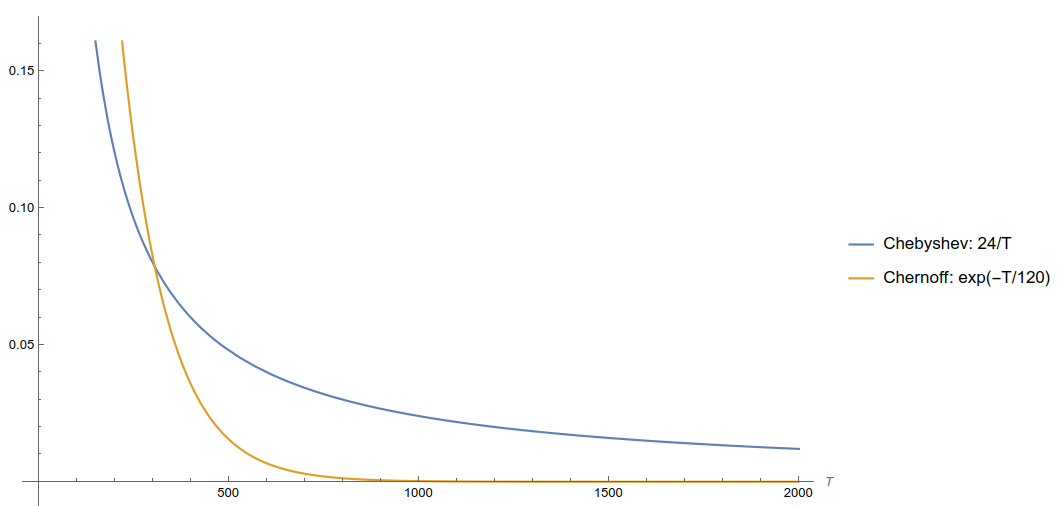
\includegraphics[width=1.25\textwidth]{figures/fig-chernoff-v-chebyshev.png}
    \caption{Bounds on $\bPr{ Y < \frac{1}{2}T }$ provided by Chebyshev's and Chernoff's inequalities, as a function of $T$.}
    \label{fig:chernoff:v:chebyshev}
\end{figure}
In any case: we wanted a failure probability less than $\errprob$? Then is suffices to solve for (integer) $T$:
\[
e^{-\frac{1}{120}T} \leq \errprob
\]
giving $T \geq \clg{120\ln(1/\errprob)}$. So with taking $T(\errprob)=O(\log(1/\errprob))$ in~\cref{algo:majority:vote} suffices to amplify the success probability of each query on $\blue{x}$ from $60\%$ to $1-\errprob$, at the (small?) cost of $O(\log(1/\errprob))$ more queries to the data structure $\red{D}$.

\begin{framed}
 We have used Markov's and Chebyshev's inequalities and the Chernoff bound, and this allowed us to analyse and amplify the success probability of our randomised algorithms. In the next lectures, we will see a related technique, also based on the Chernoff (or, looking ahead, Hoeffding) bound: a generalisation of the ``majority vote'' trick for when the output can take more than only 2 values, called the \emph{median trick.}
\end{framed}


\section{Concentration inequalities: a summary}
We summarize the ``concentration bounds''\marginnote{They are called that way because they quantify how ``concentrated'' (in terms of probability) a random variable is around its expectation.} used in the chapter so far, along with some others (more advanced) that will come in handy in the next chapters. These will be sufficient in many or most settings. 
There are, of course, \emph{many} others, and many refinements or variants of the bounds we present here. If you are interested, see \eg Chapter~2 of \cite{Vershynin18} or~\cite{BoucheronLM13} for a much more comprehensive and insightful coverage.

We start with the mother of all concentration inequalities, Markov's inequality:
\begin{theorem}[Markov's inequality]
  \label{theo:markov}
Let $X$ be a non-negative random variable with $\bEE{X} < \infty$. For any $t > 0$, we have
\[  
  \bPr{ X \geq t } \leq \frac{\bEE{X}}{t}
\]
\end{theorem}
\noindent Applying this to $(X-\bEE{X})^2$, we get 
\begin{theorem}[Chebyshev's inequality]
  \label{theo:chebyshev}
Let $X$ be a random variable with $\bEE{X^2} < \infty$. For any $t > 0$, we have
\[  
  \bPr{ \abs{X-\bEE{X}} \geq t } \leq \frac{\var[X]}{t^2}
\]
\end{theorem}
By applying Markov's inequality to the moment-generating function (MGF) of $\sum_{i=1}^n X_i$ in various ways, one can also obtain the following statements:
\begin{theorem}[Hoeffding bound]
  \label{theo:hoeffding}
Let $X_1,\dots,X_n$ be independent random variables, where $X_i$ takes values in $[a_i,b_i]$. For any $t \geq 0$, we have
\begin{align}
\bPr{ \sum_{i=1}^n X_i   > \sum_{i=1}^n \bEE{X_i} + t }  
&\leq \exp(-\frac{2 t^2}{\sum_{i=1}^n (b_i-a_i)^2}) \\
\bPr{\sum_{i=1}^n X_i  < \sum_{i=1}^n \bEE{X_i} - t }
 &\leq \exp(-\frac{2 t^2}{\sum_{i=1}^n (b_i-a_i)^2})
 \end{align}
\end{theorem}

\begin{corollary}[Hoeffding bound]
  \label{coro:hoeffding}
Let $X_1,\dots,X_n$ be \iid random variables taking value in $[0,1]$, with mean $\mu$. For any $\gamma \in (0,1]$ we have
\begin{align}
\bPr{ \abs{\frac{1}{n}\sum_{i=1}^n X_i  - \mu} > \gamma }
 &\leq 2\exp(-2 \gamma^2 n)
\end{align}
\end{corollary}

\begin{theorem}[Chernoff bound]
  \label{theo:chernoff}
Let $X_1,\dots,X_n$ be independent random variables taking value in $[0,1]$, and let $P \eqdef \sum_{i=1}^n \bEE{X_i}$ For any $\gamma \in (0,1]$ we have
\begin{align}
\bPr{\sum_{i=1}^n X_i > (1+\gamma)P } &< \exp(-\gamma^2 P/3)\\
\bPr{\sum_{i=1}^n X_i < (1-\gamma)P } &< \exp(-\gamma^2 P/2)
\end{align}
In particular, if $X_1,\dots,X_n$ are \iid with mean $\mu$, then for any $\gamma \in (0,1]$ we have
\begin{align}
\bPr{ \abs{\frac{1}{n}\sum_{i=1}^n X_i  - \mu} > \gamma\mu }
 &\leq 2\exp(-\gamma^2 n \mu/3) \label{eq:chernoff:iid}
\end{align}
\end{theorem}
As a rule of thumb, the ``multiplicative'' (Chernoff) from~\cref{theo:chernoff} is preferable to the ``additive'' bound (Hoeffding) from~\cref{coro:hoeffding} whenever $\mu  \eqdef P/n \ll 1$. In case one only has an upper or lower bound on the quantity $P = \sum_{i=1}^n \bEE{X_i}$, the following version of the Chernoff bound can come in handy:
\begin{theorem}[Chernoff bound (upper and lower bound version)]
  \label{theo:chernoff:with:ublb}
In the setting of~\cref{theo:chernoff}, suppose that
$P_L \leq P \leq P_H.$ Then for any $\gamma \in (0,1]$, we have
\begin{align}
\bPr{\sum_{i=1}^n X_i > (1+\gamma)P_H } &< \exp(-\gamma^2 P_H/3) \\
\bPr{\sum_{i=1}^n X_i < (1-\gamma)P_L } &< \exp(-\gamma^2 P_L/2)
\end{align}
\end{theorem}

%%%%%%%%%%%%%%%%%%%%%%%%%%%%%%%%%%%%%%%%%%%%%%%%%%%%%%%%%%%%%%%
\iffalse
\begin{theorem}[Bernstein's inequality] \label{theo:bernstein}
	Let $X_1,\dots, X_n$ be independent random variables taking values in $[-a,a]$, and such that $\bEE{X_i^2} \leq v_i$ for all $i$. Then, for every $t\geq 0$, we have
	\[
	\bPr{ \abs{\sum_{i=1}^n X_i-\sum_{i=1}^n \bEE{X_i}} \geq t } \leq \exp\Paren{-\frac{t^2}{2(\sum_{i=1}^n v_i+\frac{a}{3}t)}}\,.
	\]
	In particular, if $X_1,\dots,X_n$ are \iid with mean $\mu$ and $\bEE{X_1^2} \leq v$, then for any $\gamma \geq 0$ we have
	\[
	\bPr{ \abs{\frac{1}{n}\sum_{i=1}^n X_i-\mu} \geq \gamma } \leq \exp\Paren{-\frac{\gamma^2n}{2(v+\frac{a}{3}\gamma)}}\,.
	\]
\end{theorem}
Observe that this tail bound exhibits both behaviours: it decays in a subgaussian fashion for small $\gamma$, before switching to a subexponential tail bound for large $\gamma$. 

We conclude this section by providing a very convenient bound, specifically for Poisson random variables, which shares the same ``two-tail'' behaviour:
\begin{theorem}[Poisson concentration]\label{theo:main:poisson:bounds}
Let $X$ be a $\poisson{\lambda}$ random variable, where $\lambda > 0$. Then, for any $t>0$, we have
\begin{equation}\label{eq:poisson:upper:tail}
    \probaOf{ X \geq \lambda + t} \leq e^{-\frac{t^2}{2\lambda}\psi\Paren{\frac{t}{\lambda}}} \leq e^{-\frac{t^2}{2(\lambda+t)}}
\end{equation}
and, for any $0<t< \lambda$,
\begin{equation}\label{eq:poisson:lower:tail}
  \probaOf{ X \leq \lambda - t} \leq e^{-\frac{t^2}{2\lambda}\psi\Paren{-\frac{t}{\lambda}}} \leq e^{-\frac{t^2}{2(\lambda+t)}}\,,
\end{equation}
where $\psi(u)\eqdef 2\frac{(1+u)\ln(1+u)-u}{u^2}$ for $u\geq -1$.
In particular, for any $t\geq 0$,
\begin{equation}\label{eq:poisson:both:tail}
  \probaOf{ \abs{X -\lambda} \geq t} \leq 2e^{-\frac{t^2}{2(\lambda+t)}}\,.
\end{equation}
\end{theorem}
\cmargin{Is the proof needed?}
\fi